\section{Abstract Syntax Tree and Abstract Semantic Representation}

\begin{frame}{Abstract Syntax Tree (AST)}
    \begin{columns}
        \begin{column}{0.5\textwidth}
            \lstinputlisting[language=Python]{codes/simple-example.py}
            \centering Example
        \end{column}
        \begin{column}{0.5\textwidth}
            \begin{figure}
                \centering
                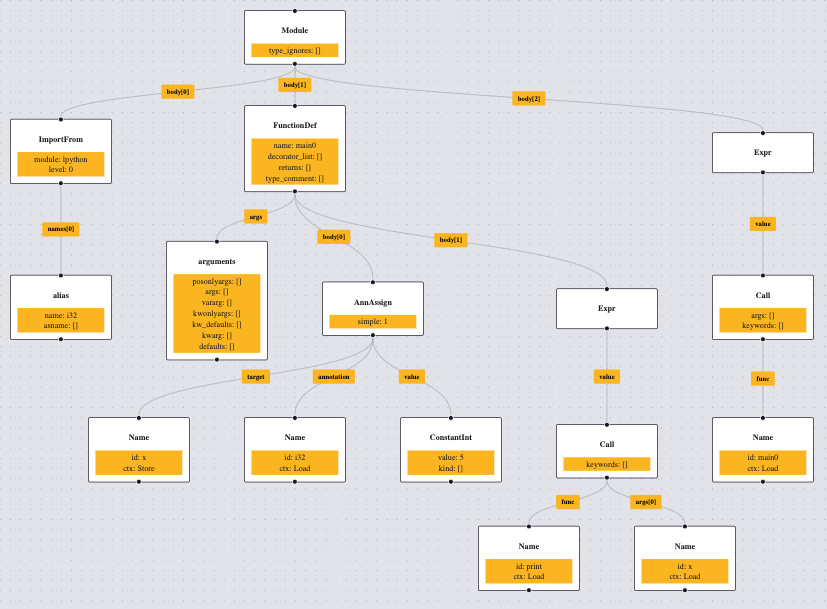
\includegraphics[width=7cm]{images/ast.png}
                \caption{AST}
            \end{figure}
        \end{column}
    \end{columns}
\end{frame}

\begin{frame}{Abstract Semantic Representation (ASR)}
    \begin{columns}
        \begin{column}{0.5\textwidth}
            \begin{figure}
                \centering
                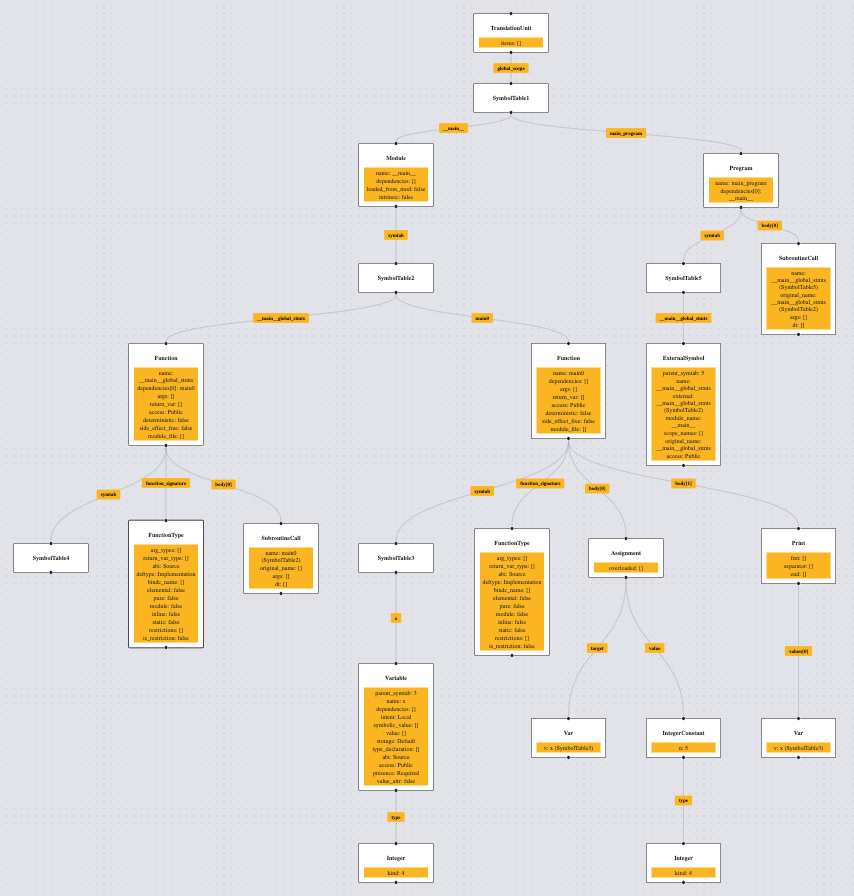
\includegraphics[width=5cm]{images/asr.png}
                \caption{ASR}
        \end{figure}
        \end{column}
        \begin{column}{0.5\textwidth}
            \begin{itemize}
                \item Independent of the frontends and backends
                \item As high level as possible, but faithful to the surface language
                \item ASR $\rightarrow$ ASR passes
                \begin{itemize}
                    \item loop vectorize
                    \item dead code removal
                    \item inline function calls, etc.
                \end{itemize}
                \item ASR $\rightarrow$ Backends
            \end{itemize}
        \end{column}
    \end{columns}
\end{frame}